\documentclass[10pt,a4paper]{article}
\usepackage[T1]{fontenc}
\usepackage[utf8]{inputenc}
\usepackage[italian]{babel}
\usepackage{times,amsmath,graphicx,booktabs}
\usepackage[top=1.8cm,bottom=1.8cm,left=1.8cm,right=1.8cm]{geometry}
\usepackage{enumitem}
\setlength{\parindent}{0pt}
\setlength{\parskip}{4pt}
\setlist{nosep,leftmargin=*}
\begin{document}
\begin{center}
{\Large Modellazione delle reti -- A.A. 2026/2027}\\[4pt]
{\large Compito 2 -- Shaping composito del traffico Zoom in uscita}\\[5pt]
Alessandro Vulcu -- Matricola 2185190, Università di Padova
\end{center}
\begin{abstract}
Implemento un token bucket seguito da un leaky bucket a velocità costante, entrambi
in tempo simulato, usando la sorgente empirica Zoom stimata nel Compito 1. Una ricerca
su griglia seleziona velocità e capacità dei buffer nel rispetto di vincoli su perdita
e ritardo. Repliche indipendenti di 30 minuti confermano la configurazione scelta.
I risultati quantificano il contributo dello shaper alla QoS per il modello di traffico
stimato, anziché la qualità complessiva della chiamata.
\end{abstract}
\section{Sorgente e implementazione}
Nel Compito 1 ho selezionato un flusso UDP Zoom in uscita, con videocamera attiva.
I primi 180 s costituiscono il campione di addestramento (19\,645 pacchetti); i successivi
120 s sono stati riservati alla validazione. Le dimensioni corrispondono alle lunghezze
delle trame Ethernet catturate, non al payload multimediale. Riutilizzo il CSV di
addestramento, con una soglia di clustering di 1 ms ed escludendo entrambi i cluster
ai bordi della traccia. I 7\,233 cicli completi risultanti sono rappresentati da
$(D_i,\{U_{i,k},L_{i,k}\}_{k=1}^{B_i})$: intervallo tra cluster, offset temporali
dei pacchetti e lunghezze. Il campionamento uniforme e indipendente di tuple complete
preserva le dipendenze tra intervallo, numero di pacchetti e lunghezze. La velocità
media stimata è 865.95 kbit/s; il pacchetto più grande misura 1\,341 B. Non occorrono
nuove catture né una nuova stima sui dati di validazione.

Per rispettare la convenzione del compito sui batch simultanei, tutti i $B_i$ pacchetti
vengono emessi all'inizio del ciclo, su righe separate con lo stesso timestamp.
L'inizio del ciclo successivo è spostato in avanti di $D_i$. Si conservano così le
distribuzioni degli intervalli tra cluster, del numero di pacchetti per batch e delle
lunghezze, eliminando deliberatamente i brevi offset interni ai cluster usati nel
Compito 1. Un'opzione separata ripristina questi offset per l'analisi di sensibilità.
La sorgente genera pacchetti in $[0,T)$ e assegna identificatori univoci consecutivi.

\texttt{source.py} genera il file di ingresso; \texttt{shaper.py} lo legge e scrive
il file di uscita. Entrambi usano tre campi separati da spazi bianchi: identificatore,
timestamp in secondi e lunghezza in byte. I tempi in ingresso sono gli istanti di
generazione; quelli in uscita sono gli istanti di completamento della trasmissione.
Identificatori e lunghezze restano invariati. Gli identificatori dei pacchetti scartati
compaiono soltanto in un registro separato degli scarti. Non si elaborano payload
e non si attende in tempo reale.

Il token bucket parte pieno, con un saldo di token a valori reali e reintegro continuo:
\[
q(t+\Delta)=\min\{b,q(t)+\rho\Delta\},\qquad
t_{\rm eligible}=t+\max\{0,L_{\rm head}-q(t)\}/\rho.
\]
Un token copre un byte. Può uscire soltanto il pacchetto in testa alla FIFO; il
trasferimento consuma un numero di token pari alla sua intera lunghezza. I pacchetti
che superano $b$ vengono scartati esplicitamente. Se i token non bastano, i pacchetti
vengono accodati nel buffer FIFO di capacità $B_i$; se manca spazio, il pacchetto
in arrivo viene scartato (tail drop). Non c'è backpressure: un pacchetto trasferito
verso una coda LBF piena viene scartato e i suoi token restano consumati. Il LBF
trasmette un pacchetto alla volta per $L/\mu$ secondi, senza interruzioni; la coda
di attesa ha capacità $B_o$. Le capacità delle code contano i byte in attesa ed
escludono il pacchetto in servizio. Un trasmettitore inattivo può quindi accettare
un pacchetto anche con $B_o=0$.

La simulazione procede per eventi: l'orologio avanza direttamente al primo tra
l'arrivo di un pacchetto, la disponibilità dei token necessari per quello in testa
alla coda e il completamento di una trasmissione. Quando più eventi coincidono,
si gestisce prima il completamento LBF, poi il trasferimento dei pacchetti già
accodati nel TBF che dispongono dei token necessari e infine i nuovi arrivi,
nell'ordine del file. Si rispetta così l'ordine FIFO, senza permettere ai nuovi
pacchetti di scavalcare quelli in attesa. Dopo l'arresto della sorgente, la
simulazione prosegue fino allo svuotamento di entrambe le code. Per evitare blocchi
dovuti alla precisione numerica, l'istante in cui diventano disponibili i token
viene arrotondato per eccesso a un tempo rappresentabile con token sufficienti
per l'intero pacchetto, senza usare una tolleranza fissa per accettare piccoli deficit.

L'implementazione supera dieci controlli automatici su tempi esatti, ordine FIFO,
overflow di entrambi i buffer, scarto dei pacchetti troppo grandi, validazione
dell'ingresso, riproduzione della sorgente e conservazione. I controlli verificano
anche l'inviluppo TBF, la gestione di piccoli deficit di token e il comportamento
con traslazioni dell'orologio fino a $10^9$ s.
\clearpage
\section{Vincoli di QoS e metodo sperimentale}
Nelle chiamate Zoom, l'attesa riduce la reattività, le variazioni del ritardo
richiedono più buffering al ricevitore e le perdite eliminano dati video.
La Tabella 1 riporta sei vincoli di QoS per il solo shaping e due misure descrittive:
velocità offerta e throughput. I vincoli lasciano margine per propagazione, altre
code, elaborazione del codec e riproduzione.

Per fissare i limiti, prendo come riferimento una cadenza ipotetica di 30 fotogrammi/s,
pari a 33.3 ms per fotogramma. Un ritardo medio $\leq30$ ms mantiene la latenza media
aggiunta sotto un intervallo tra fotogrammi. Il limite di 50 ms sul p95 ammette
al massimo 1.5 intervalli per il 95\% dei pacchetti consegnati, mentre p99 $\leq100$ ms
consente picchi rari fino a tre intervalli. Il limite di 30 ms sul p95 della variazione
del ritardo mantiene il 95\% delle variazioni tra pacchetti consegnati successivi
entro circa un intervallo e riduce il buffering necessario in riproduzione.
I limiti sulla perdita ($\leq1\%$) e sui byte consegnati ($\geq99\%$) evitano che
ritardi bassi nascondano traffico scartato o perdite selettive di pacchetti grandi.

Per ogni pacchetto consegnato $j$, il ritardo è $d_j=t_j^{\rm out}-t_j^{\rm in}$.
La variazione è $v_j=|d_j-d_{j-1}|$, calcolata tra pacchetti consegnati consecutivi
anche in presenza di perdite intermedie. Come jitter uso il 95° percentile di questa
variazione. Il throughput si ottiene dividendo per $T$ i byte la cui trasmissione
si completa in $[0,T)$. Per le percentuali di consegna e i ritardi considero anche
lo svuotamento finale delle code. I ritardi riguardano soltanto i pacchetti consegnati
e vanno quindi letti insieme alle perdite. Tutte le velocità sono calcolate sui byte
catturati.

Valuto 192 configurazioni sulla stessa traccia di 300 s, con seed 2026:
\[
\begin{aligned}
\rho&\in\{110,140,180,220\}\times10^3\ \mathrm{B/s},&
b&\in\{1341,4096,8192,16384\}\ \mathrm{B},\\
B_i&\in\{4096,16384\}\ \mathrm{B},&
\mu&\in\{120,220,300\}\times10^3\ \mathrm{B/s},\\
B_o&\in\{4096,16384\}\ \mathrm{B}.&&
\end{aligned}
\]
Usare la stessa traccia permette di isolare l'effetto dei parametri. Le configurazioni
che rispettano tutti i vincoli sono 28; tra queste scelgo quella che minimizza
l'indice normalizzato di consumo delle risorse
\[
C=\frac{\rho}{10^5}+\frac{\mu}{10^5}+\frac{b+B_i+B_o}{16384}.
\]
Le due velocità riservate e la capacità totale hanno peso unitario dopo la
normalizzazione. La capacità del bucket rappresenta il margine per i burst,
mentre quelle dei buffer misurano lo spazio di attesa. Poiché ogni risorsa ha
peso positivo, la minimizzazione seleziona una configurazione ammissibile e
non dominata all'interno della griglia.

Mantengo fissa la configurazione scelta ed eseguo dieci repliche indipendenti di
1\,800 s, con seed 3026--3035. Ogni replica contiene circa 196\,000 pacchetti,
pari a circa 72\,000 cicli campionati, e dura dieci volte la finestra di addestramento.
Includo il breve transitorio iniziale, partendo con code vuote e token bucket pieno
come all'inizio di una chiamata. Tutte e dieci le repliche rispettano i vincoli.
La Tabella 1 riporta la media delle statistiche ottenute nelle repliche e i relativi
intervalli di confidenza al 95\%, calcolati con la $t$ di Student:
$\bar x\pm t_{0.975,9}s_x/\sqrt{10}$. Per i quantili, l'intervallo si riferisce
alla media dei quantili delle singole repliche. Le unità statistiche indipendenti
sono le repliche, poiché i pacchetti sono correlati.

\begin{table}[h]
\centering\small
\caption{Conferma indipendente: medie e semiampiezze degli intervalli di confidenza al 95\%.}
\begin{tabular}{lrr}\toprule
Indicatore & Vincolo proposto & Media $\pm$ semiampiezza\\\midrule
Pacchetti persi (\%) & $\leq 1$ & $0.169 \pm 0.014$ \\
Byte consegnati (\%) & $\geq 99$ & $99.805 \pm 0.016$ \\
Ritardo medio (ms) & $\leq 30$ & $16.712 \pm 0.071$ \\
Ritardo, p95 (ms) & $\leq 50$ & $44.889 \pm 0.294$ \\
Ritardo, p99 (ms) & $\leq 100$ & $68.280 \pm 0.650$ \\
Variazione del ritardo, p95 (ms) & $\leq 30$ & $18.396 \pm 0.055$ \\
Velocità offerta (kbit/s) & Descrittivo & $865.196 \pm 1.774$ \\
Throughput in uscita (kbit/s) & Descrittivo & $863.502 \pm 1.787$ \\
\bottomrule\end{tabular}
\end{table}
\clearpage
\section{Risultati, compromessi e limiti}
I parametri selezionati sono
\[
(\rho,b,B_i,\mu,B_o)=(180000,4096,16384,220000,4096),\qquad C=5.50.
\]
La configurazione riserva 1.44 Mbit/s al TBF e 1.76 Mbit/s per la serializzazione.
I buffer offrono complessivamente 20\,480 B di spazio di attesa; aggiungendo la
capacità del bucket, il totale considerato nell'indice è 24\,576 B. Entrambe le
velocità superano il carico medio della sorgente, circa 0.866 Mbit/s, perché per
contenere il ritardo occorre gestire anche i burst brevi. Il bucket inizialmente
pieno lascia passare un piccolo burst prima di imporre la velocità di lungo periodo;
il trasmettitore ne invia poi i pacchetti in sequenza.

\begin{figure}[h]
\centering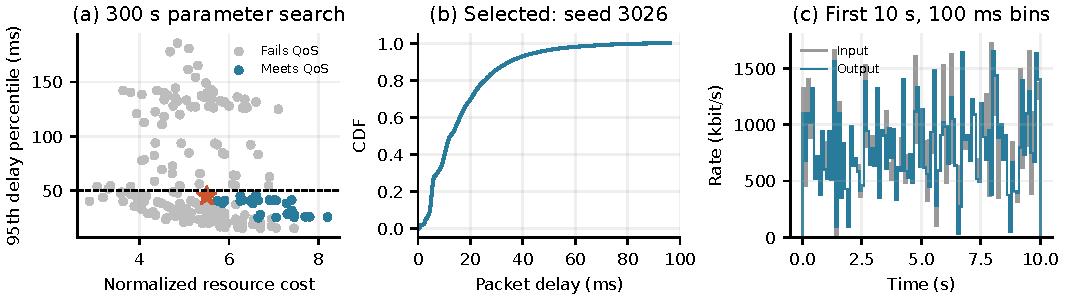
\includegraphics[width=\textwidth]{analysis/results.pdf}
\caption{Compromesso tra risorse e ritardo, distribuzione del ritardo dei pacchetti
consegnati e velocità di ingresso e uscita per la configurazione scelta. La stella
indica la configurazione ammissibile con indice minimo. Le velocità sono calcolate
su intervalli di 100 ms; i completamenti possono concentrarsi vicino ai loro bordi.}
\end{figure}

La replica rappresentativa (seed 3026) consegna 196\,181 pacchetti su 196\,556:
i 375 scarti avvengono tutti nel buffer di ingresso. L'occupazione massima è
16384 B in ingresso e 4038 B nella coda di attesa in uscita. Il buffer di uscita
può essere piccolo perché il TBF distribuisce i burst nel tempo prima di passarli
al trasmettitore, che è più veloce.

Aumentare $b$ può ridurre l'attesa in ingresso, ma riversa un burst più grande
nella coda di uscita. Un $B_i$ maggiore evita alcune perdite, al prezzo di ritardi
potenzialmente più lunghi; aumentare $B_o$, invece, non recupera i pacchetti già
scartati in ingresso. Aumentare $\rho$ riduce l'attesa dei token, mentre aumentare
$\mu$ abbrevia la serializzazione e l'attesa in uscita. L'effetto di ciascun
intervento dipende quindi dallo stadio che limita il sistema.

\begin{table}[h]
\centering\small
\caption{Casi di controllo e verifiche di robustezza, con seed 3026 per i casi sintetici.}
\begin{tabular}{lrrr}\toprule
Caso & Perdita (\%) & Ritardo p95 (ms) & Uscita (kbit/s)\\\midrule
Sottodimensionato & 29.16 & 48.98 & 587.15 \\
Buffer grandi, velocità basse & 1.10 & 546.62 & 855.08 \\
Offset intra-batch originali & 0.19 & 45.28 & 864.03 \\
Segmento di validazione di 120 s & 0.04 & 31.23 & 856.88 \\
\bottomrule\end{tabular}
\end{table}

Nel caso sottodimensionato, $(90000,1341,4096,100000,4096)$, il ritardo rimane basso
ma le perdite sono elevate. Anche la configurazione con velocità basse e buffer
grandi, $(110000,8192,65536,120000,65536)$, viola i vincoli di QoS e produce ritardi
molto maggiori: aumentare soltanto i buffer non compensa velocità insufficienti.
Ripristinando gli offset dei pacchetti del Compito 1 si ottengono risultati molto
simili a quelli della replica rappresentativa. Anche il segmento della stessa
cattura riservato alla validazione rispetta tutti i vincoli, ma la sua breve durata
non sostituisce le simulazioni più lunghe.

Gli intervalli di confidenza descrivono la variabilità delle simulazioni basate
sulla sorgente empirica stimata. Non includono l'incertezza dovuta al campione di
addestramento di 180 s, a utenti o percorsi di rete diversi e alla correlazione
temporale lenta individuata nel Compito 1. Campionando i cicli in modo indipendente
si perde questa correlazione e si sovrastima parte della variabilità su intervalli
di 100 ms. Ripetere le simulazioni non aggiunge nuove osservazioni del traffico reale.
Inoltre, lo shaper non invia segnali di congestione al codificatore adattivo di Zoom.
La scelta resta quindi legata al modello, alla griglia e al criterio di costo usati.
Per validarla in condizioni reali servirebbero altre catture e misure di qualità
end-to-end.

\textbf{Riproducibilità.} \texttt{README.md} descrive i comandi dei due moduli,
la provenienza dei dati di addestramento, gli alias delle tracce e i test.
Per riprodurre tutti gli esperimenti si esegue \texttt{python experiments.py},
seguito da \texttt{python build\_report.py}. La cartella del compito contiene
codice sorgente, tabelle dei risultati, tracce dei buffer e degli scarti,
sorgente della figura e questa relazione.
\end{document}
